\IEEEPARstart{F}{ace} recognition is a part of biometrics, as well as fingerprints, analysis of hand geometry, iris, retina and voice.
The main application field of biometrics is the access control. It provides solutions safe, cheap, simple and effective.
But in recent years, emerging biometrics in civil matters, for recreational, social and practical purposes.

\subsection{For the access control}

There are two main areas in biometrics : identification and verification.

\paragraph{In the verification or authentication} the biometric system asks the user's identity and tries to answer the question, "Is this person X? ". In an application of the verification system is reliant on biometric information from the user, and compares the data obtained from the characteristic information input with the recorded data corresponding to the asserted identity, it is a one to one comparison (1:1).

The system will find or not find a matching between the two. Verification is commonly used in applications of access control and payment authentication. Biometrics offers many advantages over existing methods of personal authentication such as keys, identification numbers (ID), passwords and swipe cards. Indeed it provided more security and convenience that generates enormous economic benefits and fills the security vulnerabilities of passwords, especially with the current facilities to perform attacks and make cracking.

Thus, these applications are used to identify a large number of people in real time. They are fast and accurate because the reference image has a good quality and image control is taken from the front in optimal conditions.

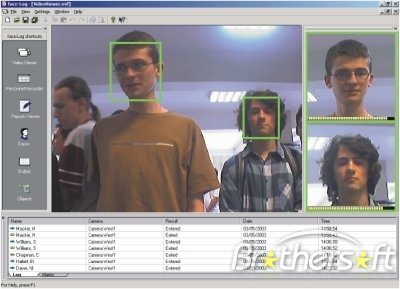
\includegraphics[width=\linewidth]{img/face_recognition_civil}
~\\
Exemples of applications : Passport verification at the airport, windows logon, access to a secure area 

\paragraph{With the identification or recognition} the biometric system asks and attempts to answer the question, "Who is the person X? ". In an identification application, the biometric device requested a biometric information and compares it with every piece of information stored in the database is a comparison to multi (1: N). The object identification applications is to identify criminals and terrorists using the surveillance data.

However, the identification of a suspect filmed by a CCTV camera where conditions are less optimal.
The image is often of poor quality, not always face, facial expression is not neutral, the brightness is different reference pictures.
Again, this time the comparison is not with a single image but with a whole database. The work to be done quickly became much more consistent.

The table~\cite{NPIA} below shows the similarity between the fingerprints searching and the face recognition.

~\\
\begin{tabular}{|p{0.28\linewidth}|p{0.28\linewidth}|p{0.28\linewidth}|}
\hline
\textbf{Fingerprints searching}&\textbf{Face Recognition}&\textbf{Capability}\\
\hline
Ten print to Ten print searching&Mugshot to Mugshot&Identification of an Live Image to Mugshot individual in custody\\
\hline
Ten print to Mark searching&Mugshot to CCTV image&Linking known individuals to unsolved crimes\\
\hline
Mark to Ten print searching&CCTV image to Mugshot&Identifying suspects from forensic evidence at crime scenes\\
\hline
Mark to Mark&CCTV images from multiple cameras&Linking unsolved crimes together\\
\hline
\end{tabular}

~\\

\subsection{Other fields}
\subsubsection*{Video Communication and Avatar Chats}
The attractiveness of today's online chat rooms is mainly derived from the secure protection of the anonymity of the chat participants allowing to talk about most private issues if desired. However, the main drawback is the pure text based communication, which lead to an invented chat-language. It comprises numerous different Smileys and *xy* codes for the expression of the emotion, which is so essential for a good communication and fewer misunderstanding.

The protection of anonymity within natural human-human video communication is another application scenario of the FEASy technology. Since the face analysis of FEASy is based on the re-synthesis of a face, the found shapes and positions of eyes, brows, mouth, etc. can be applied to any photography of a face from, say, Brad Pitt, Julia Roberts, or anybody else. Thus, today's text-chat rooms can significantly benefit from providing video chat functionality with the entertainment factor of fitting e.g. celebrities' faces to each chat partner.
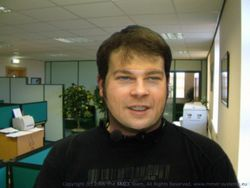
\includegraphics[width=.6\linewidth]{img/avatarchat}

\subsubsection*{Facebook}
The social network Facebook announced on Thursday, July 1, the introduction of a new facial recognition system designed to simplify the classification of images published on the site.
"This will probably surprise you, but on the pictures, people take the bulk of their time to download, browse and tag photos. We seek to improve our experience in this field, " says Sam Odio, head of Facebook on the official blog of the group.
The aim of the new device is indeed simplify the identification of these images. On each photograph, when a face is recognized automatically by the program, a window appears asking the user's social network to include the full name of the person, or any other keyword. Two months ago, the company had already acquired the sapling Divvyshot specializing in facial recognition.

\subsubsection*{NeoFace}
The solution NeoFace Nec, equips the Hong Kong Immigration Department, by matching the number plate with the driver's face, correspondence established at the time of passport application and the barrier at the border opens.

\subsubsection*{Targeted messages on billboard}
Companies like Quividi offer targeted messages solutions depending on the person viewing the billboard. The idea:
\begin{itemize}
\item You're a teenager with lots of button -> Biactol
\item You're a mom with a stroller -> Guigoz
\item A couple held hands - no alliance -> Pronuptia
\item A little old man with a cane -> Aviva, for a convention of funeral
\end{itemize}

\subsubsection*{Facelook}
Polar Rose, a Swedish company just purchased by Apple, moved to link different profiles (facebook, lastfm, twitter,...) to your face from your mobile phone.

You're on a beach in Barcelona.
A girl you like, you would like to know more about her.
You installed the application on your mobile, you point to the girl.
Face recognition allows you to find your profile.
A modern version of the sweeper.

\subsubsection*{FaceAPI}
faceAPI allows you to incorporate Seeing Machines world class face tracking technology into your own product or application. faceAPI provides a suite of image-processing modules created specifically for tracking and understanding faces and facial features. These powerful tracking modules are combined into a complete API toolkit that delivers a rich stream of information that you can incorporate into your own products or services. Seeing Machines faceAPI is the only comprehensive, integrated solution for developing products that leverage real-time face tracking. All image-processing for face tracking is handled internally, removing the need for any computer vision experience.
